\documentclass[../Chapter.tex]{subfiles}

\begin{document}

\chapter{Prime Decomposition in Number Rings}

\subsection*{Exercise 3.1}

$(1)\Rightarrow(1')$ Suppose every ideal is finitely generated. Given any ascending chain of ideals $I_1\subseteq I_2\subseteq I_3\subseteq\cdots$. Let $\Ical:=\cup_{k=1}^\infty I_k$. It's easy to check that $\Ical$ is also an ideal of $R$ and hence it's finitely generated. Write $\Ical=Rr_1+\cdots+Rr_n$ where $r_i\in I_{k_i}$. WLOG, may assume $I_{k_i}\subseteq I_{k_{i+1}}$ $\forall i=1,\ldots,n-1$. 

We claim $\Ical=I_{k_n}$. $\Ical\supseteq I_{k_n}$ is clear. Conversely, since for each $i$ we have $r_i\in I_{k_i}\subseteq I_{k_n}$, so $Rr_i\subseteq I_{k_n}$ and thus $\Ical\subseteq I_{k_n}$. This completes the claim. Since for each $k\geq k_n$, we have $I_k\subseteq \Ical=I_{k_n}$. And it's easy to see that $I_k\supseteq I_{k_n}$. Hence $I_k=I_{k_n}$. This means the ascending chain will eventually stable from $k_n$.

$(1')\Rightarrow(1'')$ Suppose the a.c.c. holds. If there exists a non-empty set $S$ of ideals s.t. $S$ has no maximal elements. Then for any $I\in S$, $\exists I'\in S$ s.t. $I\varsubsetneq I'$. Repeat this process we will get a non-stable ascending chain of ideals, a contradiction.

$(1'')\Rightarrow(1)$ Suppose every non-empty set of ideals has a maximal element. Given an ideal $I$ of $R$. Consider the set of ideals $S:=\{Rr_1+\cdots+Rr_n\mid r_1,\ldots,r_n\in I\}$. Then by assumption there exists a maximal element in $S$, say $Rr_1+\cdots+Rr_n \in S$. We claim that $Rr_1+\cdots+Rr_n=I$. (So $I$ is finitely generated.)

$Rr_1+\cdots+Rr_n\subseteq I$ is clear. Conversely, if $\exists r'\in I$ and $r'\notin Rr_1+\cdots+Rr_n$, consider $Rr_1+\cdots+Rr_n+Rr' \in S$. And since $Rr_1+\cdots+Rr_n \varsubsetneq Rr_1+\cdots+Rr_n+Rr'$, this leads to a contradiction.

\subsection*{Exercise 3.2}

Let $R$ be an integral domain with cardinality $m$. Given $\alpha\in R$, consider the subset $\{\alpha,\alpha^2,\alpha^3,\ldots,\alpha^{m+1}\}$ of $R$. Then by observing the cardinality we must have $\alpha^i=\alpha^j$ for some $1\leq i<j \leq m+1$. Since $R$ is an integral domain we can use the cancellation law. Thus $\alpha^{j-i}=1$.

\subsection*{Exercise 3.3}

Write $G=\ZZ\beta_1\oplus\cdots\oplus\ZZ\beta_n$ and consider the natural group homomorphism $\phi:\ZZ\beta_1\oplus\cdots\oplus\ZZ\beta_n \to \ZZ/m\ZZ\beta_1\oplus\cdots\oplus\ZZ/m\ZZ\beta_n$. It's easy to see that $\phi$ is surjective and $\ker\phi=mG$. So $G/mG\simeq \ZZ/m\ZZ\beta_1\oplus\cdots\oplus\ZZ/m\ZZ\beta_n$ where each $\ZZ/m\ZZ\beta_i$ is a cyclic group of order $m$.

\subsection*{Exercise 3.4}

Fix an integral basis $\{\beta_1,\ldots,\beta_n\}$ of $R$ and let $\alpha\neq 0$ be any element in $I$. Since $(\alpha)\subseteq I \subseteq R$, we know $I$ is a free abelian group of rank at most $n$. And from $(\alpha)=\alpha R=\alpha(\ZZ\beta_1\oplus\cdots\oplus\ZZ\beta_n)=\ZZ\alpha\beta_1\oplus\cdots\oplus\ZZ\alpha\beta_n$ we have $I$ has rank at least $n$. So the result follows.

\subsection*{Exercise 3.5}

\subsection*{Exercise 3.6}

\subsection*{Exercise 3.7}

Fix $m,n\in\NN$ and write $1=\alpha+\beta$ where $\alpha\in I,\beta\in J$. Raising both sides to $m+n$ powers and using binomial theorem, we have
\begin{multline*}
1=\alpha^{m+n}+\binom{m+n}{1}\alpha^{m+n-1}\beta+\cdots+\binom{m+n}{n}\alpha^m\beta^n \\ +\binom{m+n}{n+1}\alpha^{m-1}\beta^{n+1}+\cdots+\binom{m+n}{m+n-1}\alpha\beta^{m+n-1}+\beta^{m+n}
\end{multline*}
This expression can be written as $\alpha^m\cdot\jk+\beta^n\cdot\jk$ and hence $1\in I^m+J^n$.

\subsection*{Exercise 3.8}

\subsection*{Exercise 3.9 \color{red}(incomplete, missing (c))}

(a) Write $I=I_1^{\alpha_1}\cdots I_s^{\alpha_s}$ where $I_i$'s are distinct and $J=J_1^{\beta_1}\cdots J_t^{\beta_t}$ where $J_j$'s are also distinct. All of them are prime ideals in $R$. Then
\begin{align*}
IS &= (I_1S)^{\alpha_1}\cdots (I_sS)^{\alpha_s}=(I_{11}\cdots I_{1n_1})^{\alpha_1}\cdots (I_{s1}\cdots I_{sn_s})^{\alpha_s} \\
JS &= (J_1S)^{\beta_1}\cdots (J_tS)^{\beta_t}=(J_{11}\cdots J_{1m_1})^{\beta_1}\cdots (J_{t1}\cdots J_{tm_t})^{\beta_t}
\end{align*}
where all primes are now in $S$.

We first claim that $I_{ik}\neq I_{i'k'}$ if $i\neq i'$. Otherwise, if $I_{ik}=I_{i'k'}$, then from $I_{ik}$ lies over $I_i$ and $I_{i'k'}$ lies over $I_{i'}$ we have $I_{ik}$ also lies over $I_{i'}$. By Thm 20 (p. 45), we must have $I_i=I_{i'}$, a contradiction. This means if two primes come from different $I_iS$, they must be different.

Since $IS\mid JS$, by rearranging appropriately, we have $I_{11}=J_{11}$. Since $I_{11},J_{11}$ lie over $I_1,J_1$, respectively. By Them 20 again, we have $I_1=J_1$.

We claim that $I_{ik}=J_{1k'}$ iff $i=1$. Assume $I_{ik}=J_{1k'}$. Then $I_{ik}$ lies over $I_i$ and $J_1(=I_1)$. So we have $i=1$. Conversely, assume $i=1$. Since $IS\mid JS$, $I_{1k}$ must be some $J_{i'k'}$. If $I_{1k}=J_{i'k'}$ where $i'\neq 1$, then $I_{1k}$ lies over $I_1(=J_1)$ and $J_{i'}$. So $i'=1$, a contradiction.

Note that from our two claims, together with $IS\mid JS$. We know $\alpha_1\leq \beta_1$. And by repeating this argument, the result follows.

(b) Take $J:=IS\cap R$. It's easy to easy that $J$ is an ideal in $S$. Moreover, from $$JS=(IS\cap R)S\subset IS^2\cap RS=IS\cap S\subset IS$$ we have $IS\mid JS$. So by (a), $I\mid J$. Hence $J=IS\cap R\subseteq I$. Conversely, $I\subseteq IS\cap R$ is clear. So we have $I=IS\cap R$.

\subsection*{Exercise 3.10}

Let $e=e(U/P),e_1=e(U/Q),e_2=e(Q/P)$. Then $QT=U^{e_1}\cdot\jk1$, $PS=Q^{e_2}\cdot\jk2$. Observe that we have $$(QT)^{e_2}=Q^{e_2}T^{e_2}=Q^{e_2}T=U^{e_1e_2}\cdot(\jk1)^{e_2}$$ and so $$PST=PT=Q^{e_2}\cdot\jk2\cdot T=U^{e_1e_2}\cdot(\jk1)^{e_2}\cdot\jk2$$ It's remaining to show $\jk1$ and $\jk2$ have no prime divisor $U$. For $\jk1$, it follows easily from the definition. For $\jk2$, let $Q_i\subset S$ be any prime divisor of $\jk2$, we want to show that $Q_i\neq U$. This can be seen from the facts that $Q_i$ lies over $P$ and by Thm 20 (p. 45) $U$ can only lie over $Q$ and not $Q_i$, so if $Q_i=U$ then by Thm 19 (p. 44) we would have $U$ lies over $Q_i$, which is absurd.

For the inertial degree, it follows easily from the tower of field extensions $R/P\subset S/Q\subset T/U$ and the fact that $[T/U:R/P]=[T/U:S/Q]\cdot[S/Q:R/P]$.

\subsection*{Exercise 3.11}

From Thm 22(c) (p. 46) we know $\|(\alpha)\|=|\Nr(\alpha)|$. Since $(\alpha)\subseteq I \subseteq R$, by the third isomorphism theorem, we have $(R/(\alpha))/(I/(\alpha))\simeq R/I$. So $$\#(R/I)\cdot\#(I/(\alpha))=\#(R/(\alpha))$$ Hence $\|I\|=\#(R/I)\mid \#(R/(\alpha))=\|(\alpha)\|=|\Nr(\alpha)|$. The equality holds iff $\#(I/(\alpha))=1$ iff $I=(\alpha)$.

\subsection*{Exercise 3.12}

\subsection*{Exercise 3.13}

\subsection*{Exercise 3.14}

In this exercise, we will put $(*)$ whenever we quote Ex 3.9(b). Moreover, in parts (a) and (b), we will write $e=e(Q/P),f=f(Q/P)$ for the sake of simplicity. And we assume $PS=(Q_1\cdots Q_r)^e$ where $Q_i$'s are distinct primes. Note that by the Cor of Thm 23 (p. 50), we have $e=e(Q_i/P),f=f(Q_i/P)$ for all $i=1,\ldots,r$.

(a) By Thm 23 (p. 49), $\exists\phi\in G$ s.t. $\phi(Q)=Q'$. Define the map
$$
\begin{array}{ccc}
\{\sigma\mid \sigma(Q)=Q\} & \longleftrightarrow & \{\tau\mid \tau(Q)=Q'\} \\
\sigma & \longmapsto & \phi\circ\sigma \\
\phi^{-1}\circ\tau & \longmapsfrom & \tau
\end{array}
$$
It's easy to see that this is a bijection. Hence these two sets have the same cardinality.

Write $G=\cup_{i=1}^r \Gcal_i$ where $\Gcal_i:=\{\sigma\mid \sigma(Q_1)=Q_i\}$. This is clearly a disjoint union and we've shown that all $\Gcal_i$ have the same cardinality, we denote it as $g$. So $n=\#(G)=rg$. Since $n=ref$, we have $g=ef$.

(b) By $(*)$, $P^f=R\cap P^fS=R\cap(PS)^f=R\cap(Q_1\cdots Q_r)^{ef}$. So it's remaining to show $(Q_1\cdots Q_r)^{ef}=\prod_{\sigma\in G}\sigma(Q)$. WLOG, we assume $Q=Q_1$. From (a) we know there are $ef$ $\sigma$'s map $Q_1$ to $Q_i$ $\forall i=1,\ldots,r$. So $\prod_{\sigma\in G}\sigma(Q_1)=Q_1^{ef}\cdots Q_r^{ef}=(Q_1\cdots Q_r)^{ef}$.

(c) Write $I=I_1\cdots I_s$ where $I_i$'s are prime in $S$. Each $I_i$ lies over a unique prime ideal in $R$, say $J_i$. For each $i$, let $e_i,f_i$ be the corresponding ramification index and inertial degree of $I_i$ over $J_i$. Then $J_iS=(I_i\cdot\jk)^{e_i}$. So similar to (b), we have $$\prod_{\sigma\in G}\sigma(I_i)=\sigma_1(I_i)\cdots\sigma_n(I_i)=(I_i\cdot\jk)^{e_if_i}=(J_iS)^{f_i}=J_i^{f_i}S$$ Let $J:=\prod_{i=1}^s J_i^{f_i}$, then $$\prod_{\sigma\in G}\sigma(I)=\prod_{\sigma\in G}\sigma(I_1)\cdots\sigma(I_s)=\prod_{i=1}^s\left(\prod_{\sigma\in G}\sigma(I_i)\right)=\prod_{i=1}^s J_i^{f_i}S=JS$$ By $(*)$, $J=JS\cap R=\prod_{\sigma\in G}\sigma(I)\cap R=\Nr^L_K(I)$. So $JS=\prod_{\sigma\in G}\sigma(I)=\Nr^L_K(I)\cdot S$.

(d) Note that "Norm" is an ideal in $R$. So
\begin{align*}
\Nr^L_K(IJ) &\overset{(*)}{=} \Nr^L_K(IJ)\cdot S\cap R \overset{(c)}{=} \prod_{\sigma\in G}\sigma(IJ)\cap R = \prod_{\sigma\in G}\sigma(I)\sigma(J)\cap R \\
&= \prod_{\sigma\in G}\sigma(I)\prod_{\sigma\in G}\sigma(J)\cap R \overset{(c)}{=} \left(\Nr^L_K(I)\cdot S\right)\left(\Nr^L_K(J)\cdot S\right)\cap R \\
&= \Nr^L_K(I)\Nr^L_K(J)S\cap R \overset{(*)}{=} \Nr^L_K(I)\Nr^L_K(J)
\end{align*}

(e) We will use the fact that $\Nr^L_K(\alpha)\in R$.
\begin{align*}
\Nr^L_K((\alpha)) &= \Nr^L_K(\alpha S) = R\cap \prod_{\sigma\in G}\sigma(\alpha S) = R\cap \prod_{\sigma\in G}\sigma(\alpha)\sigma(S) \\
&= R\cap \Nr^L_K(\alpha)\cdot S = R\cap\left(\Nr^L_K(\alpha)\cdot R\right)\cdot S \\
&= \Nr^L_K(\alpha)\cdot R
\end{align*}

\subsection*{Exercise 3.15}

(a) Factor $I$ in the number ring of $M$: $I=I_1\cdots I_r$ where $I_i$'s are prime. By Thm 20 (p. 45), each $I_i$ lies over a unique prime ideal $Q_i$ in the number ring of $L$, and each $Q_i$ lies over a unique prime ideal $P_i$ in the number ring of $K$. So we have a tower of prime ideals $P_i\subset Q_i\subset I_i$. By Ex 3.10, $f(I_i/P_i)=f(I_i/Q_i)f(Q_i/P_i)$. So
\begin{align*}
\Nr^L_K\left(\Nr^M_L(I)\right) &= \Nr^L_K\left(\Nr^M_L\left(\prod_{i=1}^r I_i\right)\right) = \Nr^L_K\left(\prod_{i=1}^r \Nr^M_L(I_i)\right) \\ 
&= \Nr^L_K\left(\prod_{i=1}^r Q_i^{f(I_i/Q_i)}\right) = \prod_{i=1}^r \left(\Nr^L_K(Q_i)\right)^{f(I_i/Q_i)} = \prod_{i=1}^r \left(P_i^{f(Q_i/P_i)}\right)^{f(I_i/Q_i)} \\
&= \prod_{i=1}^r P_i^{f(Q_i/P_i)f(I_i/Q_i)} = \prod_{i=1}^r P_i^{f(I_i/P_i)} = \prod_{i=1}^r \Nr^M_K(I_i) = \Nr^M_K(I)
\end{align*}

(b) Let $M$ be the normal closure of $L$ over $K$. Then we have a tower of field extensions $K\subset L\subset M$. By field theory since $M/K$ is normal, we have $M/L$ is also normal. Let $R,S,T$ be the number rings of $K,L,M$, respectively. Our goal is to show $\Nr^L_K(\alpha S)=\Nr^L_K(\alpha)R$.

Write $\alpha S=Q_1\cdots Q_r$ where $Q_i$'s are prime in $S$. Then $\alpha S\cdot T=Q_1T\cdots Q_rT$. For each $i=1,\ldots,r$, since $M/L$ is normal, we may write $Q_iT=(I_{i1}\cdots I_{in_i})^{e_i}$ where $I_{i1},\ldots,I_{in_i}$ are prime in $T$. Let $f_i$ be the corresponding inertial degree, then by (a)
\begin{align*}
\Nr^M_K(Q_iT) &= \Nr^L_K\left(\Nr^M_L(Q_iT)\right) = \Nr^L_K\left(\Nr^M_L\left(\prod_{k=1}^{n_i} I_{ik}^{e_i}\right)\right) \\
&= \Nr^L_K\left(\prod_{k=1}^{n_i}\left(\Nr^M_L (I_{ik})^{e_i}\right)\right) = \Nr^L_K\left(\prod_{k=1}^{n_i} Q_i^{e_if_i}\right) \\
&= \Nr^L_K\left(Q_i^{e_if_in_i}\right) = \Nr^L_K\left(Q_i^{[M:L]}\right) = \Nr^L_K(Q_i)^{[M:L]}
\end{align*}
So
\begin{align*}
\Nr^M_K(\alpha S\cdot T) &= \Nr^M_K\left(\prod_{i=1}^r Q_iT\right) = \prod_{i=1}^r \Nr^M_K(Q_iT) = \prod_{i=1}^r \Nr^L_K(Q_i)^{[M:L]} \\
&= \Nr^L_K\left(\prod_{i=1}^r Q_i\right)^{[M:L]} = \Nr^L_K(\alpha S)^{[M:L]}
\end{align*}
On the other hand, since $M/K$ is normal, by Ex 3.14 (e), we have
\begin{align*}
\Nr^M_K(\alpha S\cdot T) &= \Nr^M_K(\alpha T) = \Nr^M_K(\alpha)R = \Nr^L_K\left(\Nr^M_L(\alpha)\right)R \\
&= \Nr^L_K\left(\alpha^{[M:L]}\right)R = \left(\Nr^L_K(\alpha)\right)^{[M:L]}R = \left(\Nr^L_K(\alpha)R\right)^{[M:L]} 
\end{align*}
We've used the fact that $\alpha\in S$ in the fourth equality.

Combining these two gives us $\Nr^L_K(\alpha S)^{[M:L]}=(\Nr^L_K(\alpha)R)^{[M:L]}$. They are ideals in $R$. Hence $\Nr^L_K(\alpha S)=\Nr^L_K(\alpha)R$ by the unique factorization of prime ideals.

(c) First we assume $I=Q$ is a prime. Then $Q$ lies over a unique prime ideal $(p)=p\ZZ$ in $\ZZ$. Let $f=f(Q/p\ZZ)$, then $\Nr^L_\QQ(Q)=(p\ZZ)^f=p^f\ZZ=\#(S/Q)\cdot\ZZ=\|Q\|\cdot\ZZ$.

In general, write $I=Q_1\cdots Q_r$ where $Q_i$'s are prime. Then $\Nr^L_\QQ(I)=\Nr^L_\QQ(Q_1\cdots Q_r)=\Nr^L_\QQ(Q_1)\cdots\Nr^L_\QQ(Q_r)=\|Q_1\|\ZZ\cdots\|Q_r\|\ZZ=\|Q_1\cdots Q_r\|\ZZ=\|I\|\ZZ$.

\subsection*{Exercise 3.16}

(a) Define $\phi:G(S)\to G(R)$ by $\phi([I])=[\Nr^L_K(I)]$ where $I$ is a prime ideal in $S$. We only check this is well-defined because $\phi$ is clearly a group homomorphism. Given two ideals $I,J$ in $S$ where $[I]=[J]$, $\exists a,b\in S$ s.t. $aI=bJ\implies aS\cdot I=bS\cdot J\implies \Nr^L_K(aS)\Nr^L_K(I)=\Nr^L_K(bS)\Nr^L_K(J)$. By Ex 3.15(b), we have $\Nr^L_K(aS)=\Nr^L_K(a)\cdot R=:(\alpha)$ and $\Nr^L_K(bS)=\Nr^L_K(b)\cdot R=:(\beta)$ where $\alpha,\beta\in R$. So $\alpha\cdot\Nr^L_K(I)=\beta\cdot\Nr^L_K(J)$ and hence $[\Nr^L_K(I)]=[\Nr^L_K(J)]$.

(b) Let $f:=f(Q/P)$. From group theory we know $\ord(\phi([Q]))\mid \ord([Q])$. Also note that $\phi([Q])=[\Nr^L_K(Q)]=[P^f]=[P]^f$. Thus $$d_P=\ord([P])\mid \ord([P]^f)\cdot f = \ord(\phi([Q]))\cdot f\mid \ord([Q])\cdot f=d_Q\cdot f$$

\subsection*{Exercise 3.17}

(a) We know $f(Q/(2))=f(Q/P)f(P/(2))$. By Thm 25 (p. 52) we have $f(P/(2))=1$. On the other hand, by Thm 26 (p. 53), $f(Q/(2))$ equals the order of $2$ in $(\ZZ/23\ZZ)^{\times}$, which is $11$. Thus, $f(Q/P)=11$.

By observing the degrees of the tower of field extensions $\QQ\subset \QQ(\sqrt{-23})\subset \QQ(\omega)$, we have $\phi(23)=22=[\QQ(\omega):\QQ(\sqrt{-23})]\cdot 2$, so $[\QQ(\omega):\QQ(\sqrt{-23})]=11$. And since $f(Q/P)=11$, by Thm 21 (p. 46) we have $P\ZZ[\omega]=(2,\theta)\ZZ[\omega]=Q$.

(b) We first show that $$P^3=\left(8,2+2\sqrt{-23},-11+\sqrt{-23},\frac{-17-5\sqrt{-23}}{2}\right)=\left(\frac{-3+\sqrt{-23}}{2}\right)=(\theta-2)$$ This is straightforward by simple calculation, observe that
\begin{align*}
2+2\sqrt{-23} &= \left(\frac{-3+\sqrt{-23}}{2}\right)\left(\frac{5-\sqrt{-23}}{2}\right) \\
\frac{-17-5\sqrt{-23}}{2} &= \left(\frac{-3+\sqrt{-23}}{2}\right)(-2+\sqrt{-23})
\end{align*}
and on the other hand, $$\frac{-3+\sqrt{-23}}{2}=(8)(-4)+(-11+\sqrt{-23})(-2)+\left(\frac{-17-5\sqrt{-23}}{2}\right)(-1)$$ So we have $P^3=(\theta-2)$

We next show that $P$ is not principal in $R$, if $P=(2,\theta)=(\alpha)=\alpha R$ is principal, then by Thm 22(c) (p. 46), $\|(\alpha)\|=|\Nr^K_\QQ(\alpha)|$. It's easy to see that $\|(\alpha)\|=\#(R/(2,\theta))=2$. (See the argument on p. 42.) So $\Nr^K_\QQ(\alpha)=\pm 2$.

On the other hand, since $\alpha\in R$, write $\alpha=a+b((1+\sqrt{-23})/2)$ where $a,b\in\ZZ$. So $\Nr^K_\QQ(\alpha)=a^2+ab+6b^2=\pm 2$. We claim that this is impossible by showing that this equation has no integral solutions.

Suppose $(a,b)$ is an integral solution, if none of $a,b$ is zero, then $a^2+6b^2\geq 7$, so $\pm2 = a^2+ab+6b^2 \geq 7+ab$. From this we get $-ab\geq 5,9$. Observe that
\begin{align*}
\pm2 = a^2+ab+6b^2 = (a+b)^2+5b^2-ab \geq -ab \geq 5,9
\end{align*}
This is a contradiction, so we have at least one of $a,b$ is zero. But this is impossible by simple calculation. Hence $a^2+ab+6b^2=\pm2$ has no integral solutions.

(c) If $Q$ is principal, then $[Q]$ is the identity element in $G(\ZZ[\omega])$. By (a) and Ex 16(b), $d_P\mid d_Q\cdot f(Q/P)=1\cdot 11$. So $d_P=1,11$. By (b) we have $P$ is not principal, so $d_P=11$. This is a contradiction because by (b) we know $[P]^3=[(\theta-2)]$ so $d_P=3$.

(d) By (a) we know $f(Q/P)=11$. And since $2\nmid 23$, by the Cor of Thm 26 (p. 54), $2\ZZ[\omega]=(\alpha\beta)=(\alpha)(\beta)$ is the product of two prime ideals. We know one of them is $Q$. And by (c), $Q$ is not principal, so $Q\neq (\alpha)$ and $Q\neq(\beta)$. This means one of $(\alpha),(\beta)$ must be able to be factorized further. WLOG, say $(\alpha)$. So $(\alpha)=QQ'$ for some $Q'$. In this case, $(\beta)=\ZZ[\omega]$, i.e., $\beta$ is a unit.

\subsection*{Exercise 3.18}

Let $\sigma_1,\ldots,\sigma_n$ be the $n$ embeddings of $K$ into $\CC$. For each $j=1,\ldots,n$, we write $\sigma(\alpha_j):=(\sigma_1(\alpha_j),\ldots,\sigma_n(\alpha_j))^T\in K^n$.

(a) We use the fact that the determinant is multilinear. Thus,
\begin{align*}
\disc(r\alpha_1,\alpha_2,\ldots,\alpha_n) &= |\sigma(r\alpha_1),\sigma(\alpha_2),\ldots,\sigma(\alpha_n)|^2 \\
&= |r\sigma(\alpha_1),\sigma(\alpha_2),\ldots,\sigma(\alpha_n)|^2 \\
&= r^2|\sigma(\alpha_1),\sigma(\alpha_2),\ldots,\sigma(\alpha_n)|^2 \\
&= r^2\disc(\alpha_1,\ldots,\alpha_n)
\end{align*}

(b) We use the fact that the determinant remains unchanged under the operation of adding a scalar multiple of one column to another column. Since $\beta$ is a linear combination of $\alpha_2,\ldots,\alpha_n$ over $\QQ$. We know $\sigma_i(\beta)$ is a linear combination of $\sigma_i(\alpha_2),\ldots,\sigma_i(\alpha_n)$ over $\QQ$ for all $i$. Thus,
\begin{align*}
\disc(\alpha_1+\beta,\alpha_2,\ldots,\alpha_n) &= |\sigma(\alpha_1+\beta),\sigma(\alpha_2),\ldots,\sigma(\alpha_n)|^2 \\
&=|\sigma(\alpha_1)+\sigma(\beta),\sigma(\alpha_2),\ldots,\sigma(\alpha_n)|^2  \\
&= |\sigma(\alpha_1),\sigma(\alpha_2),\ldots,\sigma(\alpha_n)|^2 \\
&= \disc(\alpha_1,\ldots,\alpha_n)
\end{align*}

\subsection*{Exercise 3.19}

(a) Assume $\alpha\notin PS$. Since $S/PS$ is a vector space over $R/P$ with dimension $n=[L:K]$ (see p. 48). Let $\{\gamma_1,\ldots,\gamma_n\}\subset S$ s.t. the corresponding elements in $S/PS$ form a basis of $S/PS$ over $R/P$. Since $\alpha\notin PS$, we may write $\alpha=c_1\gamma_1+\cdots+c_n\gamma_n$ where not all $c_i \equiv 0 \pmod{P}$. Denote it as $c_{i_0}$, i.e., $c_{i_0}\notin P$. On the other hand, from $\alpha\beta=c_1\beta\gamma_1+\cdots+c_n\beta\gamma_n$ and since $\alpha\beta\in PS$, we have $c_i\beta \equiv 0 \pmod{P}$ $\forall i$. In particular, $c_{i_0}\beta\equiv 0 \pmod{P}$. So $c_{i_0}\beta\in P$. Since $P$ is a prime ideal and $c_{i_0}\notin P$, we have $\beta\in P$.

We provide another proof using the fact that $P$ is a maximal ideal of $R$. Assume $\beta\notin P$. By maximality of $P$ we have $R=P+(\beta)$. Write $1=p+\beta r$ where $p\in P,r\in R$. Then $\alpha=p \alpha+\alpha\beta r$. Note that $p\alpha\in PS$ and since $\alpha\beta\in PS$, we also have $\alpha\beta r\in PS$. Hence $\alpha\in PS$.

(b) By the Lem in the proof of Thm 22(b) (p. 48), take $A=P,B=(\beta,\beta_1,\ldots,\beta_n)$, $\exists\gamma\in K$ s.t. $\gamma B\subset R$ and $\gamma B \not\subset A=P$. Then we have $\gamma\beta\notin P$ or $\gamma\beta_i\notin P$ for some $i$. Note that in both cases we always have $\gamma\beta,\gamma\beta_i \in R$ for all $i$.

If the latter case occurs then we are done, so suppose $\gamma\beta_i\in P$ $\forall i$, then we must have $\gamma\beta\in R\setminus P$. Since $\alpha\notin PS$, by (a) we have $\alpha\beta\gamma=\alpha_1\beta_1\gamma+\cdots+\alpha_n\beta_n\gamma\notin PS$, which is absurd.

(c) (The idea of the proof is very similar to the proof of Thm 24 (p. 50).) Suppose $e(Q/P)>1$ where $Q$ is a prime in $S$ lying over $P$. Write $PS=QJ\varsubsetneq J$ where $J$ is divisible by all primes of $S$ lying over $P$. Take $\alpha\in J\setminus PS$, then $\alpha$ is in every prime of $S$ lying over $P$, but not in $PS$.

Write $\alpha=\alpha_1\beta_1+\cdots+\alpha_n\beta_n$ where $\beta_n\in K$. By Ex 2.25, $\exists m\in\ZZ$ s.t. $m\beta_i\in R$ $\forall i$. Then $\alpha m=\alpha_1\beta_1m+\cdots+\alpha_n\beta_nm$. Since $\alpha\notin PS$. By (b), $\exists\gamma\in K$ s.t. $\gamma m\in R$, $\gamma\beta_im\in R$ for all $i$ and $\gamma\beta_i m\notin P$ for some $i$. WLOG, may assume $\gamma\beta_1m\notin P$.

Let $\sigma_1,\ldots,\sigma_n$ be the embeddings of $L$ in $\CC$ which fix $K$. Extend them to automorphisms of some extension $M$ of $L$ which is normal over $K$. Set $d=\disc^L_K(\alpha_1,\ldots,\alpha_n)$, then similar to Ex 3.18, we have $\disc^L_K(\alpha m\gamma,\alpha_2,\ldots,\alpha_n)=(\gamma\beta_1 m)^2d$. Since $(\gamma\beta_1m)^2\notin P$, it's remaining to show $\disc^L_K(\alpha m\gamma,\alpha_2,\ldots,\alpha_n)\in P$ (using the property of prime ideal). 

Let $I$ be any prime in $T$, the number ring of $M$, lying over $P$. Note that $P\subset I\cap S$, so $I\cap S$ is a prime of $S$ lying over $P$. And since $\alpha$ is in every prime of $S$ lying over $P$. We have $\alpha\in I\cap S\subset I$. This means $\alpha$ is in every prime of $T$ lying over $P$. Moreover, for each $\sigma_i$, since $\sigma_i^{-1}(I)$ is still a prime in $T$ lying over $P$, we have $\alpha\in \sigma_i^{-1}(I)$. So $\sigma_i(\alpha)\in I$. And since $\gamma m\in R$, we have $\gamma m\sigma_i(\alpha)=\sigma_i(\gamma m\alpha)\in I$. This shows that $\disc^L_K(\alpha m\gamma,\alpha_2,\ldots,\alpha_n)\in I$. This number is automatically in $R$ because it's the discriminant of the elements in $S$. Hence, $\disc^L_K(\alpha m\gamma,\alpha_2,\ldots,\alpha_n)\in I\cap R=P$, as desired.

\subsection*{Exercise 3.20}

Let $B_i:=\{\beta^{(i)}_1,\ldots,\beta^{(i)}_{f_i}\}$ and consider $$\sum_{i,j,k} c_{ijk}\alpha_{ij}\beta^{(i)}_k=s\in PS$$ where $c_{ijk}\in R$ and the sum is taken over all $1\leq i\leq r,1\leq j\leq e_i,1\leq k\leq f_i$. Now fix an index $i$. We want to show all $c_{ijk}\in P$, so when we mod $P$, the corresponding elements of $\alpha_{ij}\beta^{(i)}_k$ are linearly independent over $R/P$.

Consider the equation mod $Q_i$. Since among all $\alpha_{ij}$, only $\alpha_{i1}\notin Q_i$. So we get $$c_{i11}\alpha_{i1}\beta^{(i)}_1+\cdots+c_{i1f_i}\alpha_{i1}\beta^{(i)}_{f_i}\equiv0\pmod{Q_i}$$ Note that since the corresponding quotient ring is a field, so we can cancel out $\alpha_{i1}$. Moreover, since $\{\beta^{(i)}_1,\ldots,\beta^{(i)}_{f_i}\}$ corresponds a basis for $S/Q_i$ over $R/P$, we have $c_{i11}=\cdots=c_{i1f_i}\in P$.

Now consider the equation mod $Q^2_i$. Since among all $\alpha_{ij}$, only $\alpha_{i1},\alpha_{i2}\notin Q^2_i$. So we get $$c_{i11}\alpha_{i1}\beta^{(i)}_1+c_{i21}\alpha_{i2}\beta^{(i)}_1+\cdots+c_{i1f_i}\alpha_{i1}\beta^{(i)}_{f_i}+c_{i2f_i}\alpha_{i2}\beta^{(i)}_{f_i}\equiv0\pmod{Q^2_i}$$ First note that since $c_{i11}=\cdots=c_{i1f_i}\in P$, we have $c_{i11}\alpha_{i1},\ldots,c_{i1f_i}\alpha_{i1}\in PS\subset Q^2_i$, so the corresponding terms disappear. Also, we know $Q_i^2\subset Q_i$. These give us $$c_{i21}\alpha_{i2}\beta^{(i)}_1+\cdots+c_{i2f_i}\alpha_{i2}\beta^{(i)}_{f_i}\equiv0\pmod{Q_i}$$ And using the same argument in the first step, we have $c_{i21}=\cdots=c_{i2f_i}\in P$.

Since the same holds for each $i$, and by repeating this process, we now know all $c_{ijk}\in P$, this completes the proof. 

\subsection*{Exercise 3.21 \color{red}(incomplete, missing (b))}

(a) We first claim that $\alpha_1,\ldots,\alpha_n$ are linearly independent over $\ZZ$. (This would imply $G$ is free with rank $n$.) Consider $c_1\alpha_1+\cdots+c_n\alpha_n=0$ where $c_i\in\ZZ$. Since $\alpha_1,\ldots,\alpha_n$ are independent mod $p$, we have $c_i\in p\ZZ$ for all $i$. We then dividing both sides by $p$, the coefficients are still integers and thus still in $p\ZZ$. Repeat the same argument we have $p^k\mid c_i$ $\forall k\in\NN$. This forces all $c_i$ to be 0.

Write $G=\ZZ\alpha_1\oplus\cdots\oplus\ZZ\alpha_n$. By Ex 2.27 (a), $\#(S/G)<\infty$. If $p\mid \#(S/G)$, then by Cauchy's theorem, $\exists s+G\in S/G$ with order $p$. Then $ps+G=0+G$ in $S/G$, i.e., $ps\in G$. Write $ps=m_1\alpha_1+\cdots+m_n\alpha_n$ where $m_i\in\ZZ$. Since $\alpha_1,\ldots,\alpha_n$ are independent mod $p$ and $ps\in pS$, we have $m_i\in p\ZZ$ for all $i$. By dividing both sides by $p$ we get $s=m_1'\alpha_1+\cdots+m_n'\alpha_n$ where $m'_i\in\ZZ$. So $s\in G$ and thus $s+G$ is the identity element in $S/G$, which is absurd.

By Ex 2.27 (c), $\disc(\alpha_1,\ldots,\alpha_n)=\disc(G)=\#(S/G)^2\disc(S)$. And from $p\nmid \#(S/G)$ we have $p\nmid \#(S/G)^2=m$.

\subsection*{Exercise 3.22}

\subsection*{Exercise 3.23}

(3.2) Suppose $m\equiv 3\pmod{4}$. This means $R=\ZZ[\sqrt{m}]$. We want to show $2R=(2,1+\sqrt{m})^2=(4,2+2\sqrt{m},m+1+2\sqrt{m})$. $\supseteq$ is clear. (Note that $m+1$ is even.) On the other hand,
since $(m+1+2\sqrt{m})-(2+2\sqrt{m})=m-1\in\rhs$, so is $\gcd(4,m-1)=2$. So we get $\subseteq$.

(3.3) Suppose $m\equiv 1\pmod{8}$. This implies $m\equiv 1\pmod{4}$ and so $R=\ZZ[{(1+\sqrt{m})/2}]$. We want to show $2R=(2,(1+\sqrt{m})/2)(2,(1-\sqrt{m})/2)=(4,1-\sqrt{m},1+\sqrt{m},(1-m)/4)$. $\supseteq$ is clear. (Note that $(1-m)/4$ is even.) On the other hand, from $(1-\sqrt{m})+(1+\sqrt{m})=2\in\rhs$, we get $\subseteq$.

Since $2\nmid m=\disc(R)$. By Thm 24 (p. 50), $2$ is unramified in $R$. So the two factors are distinct.

(3.5) Suppose $p\nmid m$ is odd and $m\equiv n^2\pmod{p}$. We want to show $pR=(p,n+\sqrt{m})(p,n-\sqrt{m})=(p^2,pn-p\sqrt{m},pn+p\sqrt{m},n^2-m)$. $\supseteq$ is clear. (Note that $p\mid n^2-m$.) On the other hand, from $(pn-p\sqrt{m})+(pn+p\sqrt{m})=2pn\in\rhs$, so is $\gcd(p^2,2pn)=p$. (Here we've used the the facts that $p$ is odd, and since $p\nmid m,p\mid n^2-m$, we must have $p\nmid n$.) So we get $\subseteq$.

Since $p\nmid m$ is odd, we know $p\nmid\disc(R)=m,4m$. By Thm 24 again, $p$ is unramified in $R$. So the two factors are distinct.

(3.4) Suppose $m\equiv 5\pmod{8}$. This implies $m\equiv 1\pmod{4}$ and so $R=\ZZ[{(1+\sqrt{m})/2}]$. Consider the polynomial $$f(x)=x^2-x+\frac{1-m}{4}\in\ZZ[x]$$ Since $f((1+\sqrt{m})/2)=0$, $f$ has a root in $R$, and so a root in $R/P$. On the other hand, $\ovl{f}(x)=x^2+x+1\in\ZZ/2\ZZ[x]$ has no root in $\ZZ/2\ZZ$. So $R/P\not\simeq\ZZ/2\ZZ$.

\subsection*{Exercise 3.24 \color{red}(incomplete, missing (c))}

(a) Let $M$ be any intermediate field of $K$ and $L$ with corresponding number ring $T$. Let $I:=Q\cap T$ be the unique prime ideal in $T$ lying under $Q$. Since $I\cap R=Q\cap T\cap R=Q\cap R=P$, so $I$ lies over $P$. Moreover, if $I'$ is another prime ideal in $T$ lying over $P$, then from $Q^n=PS\subset I'S$ we have $I'S\mid Q^n$, this means $I'S$ is the power of $Q$. In particular, $Q$ lies over $I'$. So $I=I'$. This shows that $I$ is the unique prime in $T$ lying over $P$. So $PT$ is the power of $I$. And from $1=f(Q/P)=f(Q/I)f(I/P)$ we get $f(I/P)=1$. Hence, $PT=I^{[M:K]}$. (We've used Thm 21 (p. 46) repeatedly.)

(b) Set $M:=L\cap L'$ with corresponding number ring $T$. Clearly $K\subset M$. We may consider the following diagram of field extensions
\begin{center}
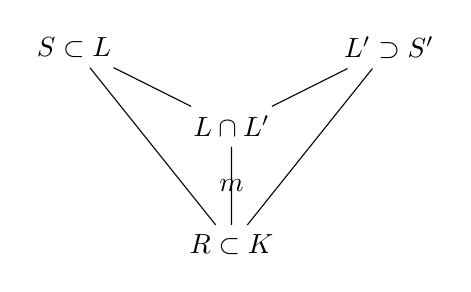
\begin{tikzpicture}
\draw (0,-0.5) node (K) {$R\subset K$};
\draw (-2,2) node (A) {$S\subset L$};
\draw (2,2) node (B) {$L'\supset S'$};
\draw (0,1) node (M) {$L\cap L'$};
\draw (M) -- (A) -- (K) --node {$m$}  (M) -- (B) -- (K);
\end{tikzpicture}
\end{center}
It's sufficient to show $m:=[M:K]=1$. Since $P$ is totally ramified in $L$, by (a), $P$ is totally ramified in $M$. So $PT=I^m$ for some prime ideal $I$ in $T$. This means $e(I/P)=m$.

On the other hand, since $P$ is unramified in $L'$, we may write $PS'=Q'_1\cdots Q'_r$. ($S'$ is the number ring of $L'$.) Observe that $I^mS'=PTS'=PS'=Q'_1\cdots Q'_r$, so we have $Q'_1\cdots Q'_r\mid I^mS'=(IS')^m$. This gives us $Q'_i\mid IS'$ and so $Q'_i$ lies over $I$ for all $i=1,\ldots,r$. Fix $i$ and from $1=e(Q'_i/P)=e(Q'_i/I)e(I/P)=e(Q'_i/I)\cdot m$, we may conclude that $m=1$.

%(c) First we consider the case $m=p^r,\omega=e^{2\pi i/m}$. Since $(p)=p\ZZ[\omega]=(1-\omega)^{\phi(m)}$, by Thm 22(a) (p. 46), we have $\|(1-\omega)\|^{\phi(m)}=\|(1-\omega)^{\phi(m)}\|=\|p\ZZ[\omega]\|=p^{[\QQ(\omega):\QQ]}$. Let $f:=f((1-\omega)/p)$, then $\|(1-\omega)\|=p^f$. So $\|(1-\omega)\|^{\phi(m)}=p^{f\phi(m)}=p^{[\QQ(\omega):\QQ]}$. This tells us $[\QQ(\omega):\QQ]\geq\phi(m)$. On the other hand, by the simple observation on p. 12 saying that the only candidates for the conjugates of $\omega$ are the $\omega^k$ where $1\leq k\leq m,\gcd(k,m)=1$. This means $[\QQ(\omega):\QQ]\leq\phi(m)$. Hence, we have $[\QQ(\omega):\QQ]=\phi(m)$. (Note that all the facts we've used didn't assume that $[\QQ(\omega):\QQ]=\phi(m)$.)

\subsection*{Exercise 3.25}

(a) Write $f(x)=\sum_{i=0}^n a_ix^i,g(x)=\sum_{i=0}^m b_ix^i$. WLOG, assume $n\geq m$. Then $\ovl{f}=\ovl{g}$ iff $a_i\equiv b_i\pmod{I}$ for $i=1,\ldots,m$ and $a_i\equiv 0\pmod{I}$ for $i=m+1,\ldots,n$ iff $a_i-b_i\in I$ for $i=1,\ldots,m$ and $a_i\in I$ for $i=m+1,\ldots,n$ iff $f-g\in I[x]$.

(b) $\ovl{g}\mid\ovl{f}$ iff $\ovl{f}=\ovl{g}\cdot\ovl{h}$ for some $\ovl{h}\in (R/I)[x]$ iff $f-gh\in I[x]$ for some $h\in R[x]$ iff $f\in(I,g)$. (We've used (a) in the second iff.)

(c) Consider the canonical ring homomorphism $\phi:R[x]\to(R/I)[x]/(\ovl{g})$ where $\phi(f):=\ovl{f}+(\ovl{g})$. This is clearly surjective. Moreover, $f\in\ker\phi$ iff $\ovl{f}+(\ovl{g})=0$ in $(R/I)[x]/(\ovl{g})$ iff $\ovl{f}\in(\ovl{g})$ iff $\ovl{g}\mid\ovl{f}$ iff $f\in(I,g)$. (We've used (b) in the last iff.) So $\ker\phi=(I,g)$. Hence we have $R[x]/(I,g)\simeq (R/I)[x]/(\ovl{g})$.

\subsection*{Exercise 3.26 \color{red}(incomplete, missing (e))}

(a) We've found an integral basis of $R$ in Ex 2.41 (or just see the application of Thm 13 (p. 28).) Using this together with Thm 6 (p. 18), it's easy to find that $\disc(R)=-27m^2/k^2$ when $m\not\equiv \pm1 \pmod{9}$, and
$-3m^2/k^2$ when $m\equiv \pm1 \pmod{9}$. (Write $m=hk^2$ where $h,k$ are relatively prime and square-free.)

From Ex 2.41(a) we know $\disc(\ZZ[\alpha])=-27m^2$. So using the formula in Ex 2.27(c), we obtain $\#(R/\ZZ[\alpha])=k$ when $m\not\equiv \pm1 \pmod{9}$, and $3k$ when $m\equiv \pm1 \pmod{9}$.

Now, suppose $p\neq 3$ is a prime and $p^2\nmid m=hk^2$. For $p\nmid m$ we have $p\nmid k,3k$. And for $p\mid m$, this implies $p\mid h$, so we have $p\nmid k,3k$. By Thm 27 (p. 55) we can decompose $pR$ by factoring $\Irr_\QQ(\alpha)=x^3-m$ in $(\ZZ/p\ZZ)[x]$.

(b) Since $\ZZ[\gamma]=\ZZ[\alpha^2/k]=\langle1,\alpha^2/k,m\alpha/k^2\rangle_\ZZ$, using Thm 6 (p. 18) again we can easily find that $\disc(\ZZ[\gamma])=\disc(1,\alpha^2/k,m\alpha/k^2)=-27m^4/k^6$. So using the formula in Ex 2.27(c) again, we obtain $\#(R/\ZZ[\gamma])=h$ when $m\not\equiv \pm1 \pmod{9}$, and $3h$ when $m\equiv \pm1 \pmod{9}$.

Now, suppose $p^2\mid m=hk^2$. This implies $p\mid k$ and $p\nmid h$, so when $p\neq 3$ we have $p\nmid h,3h$. On the other hand, when $p=3$, this implies $9\mid m$. So we have $m\equiv 0\not\equiv \pm 1\pmod{9}$. In this case, $p=3\nmid h$.

$g=\Irr_\QQ(\gamma)=\Irr_\QQ(\alpha^2/k)=x^3-h^2k$. From $p\mid k$ we have $\ovl{g}=x^3\in(\ZZ/p\ZZ)[x]$. So by Thm 27, $pR=(p,\gamma)^3=(p,\alpha^2/k)^3$.

(c) Suppose $m\not\equiv \pm1\pmod{9}$ and consider $p=3$. If $3$ divides $m$ exactly two times, this implies $3^2\mid m$. So by (b), $3R=(3,\alpha^2/k)^3$. On the other hand, for $3$ divides $m$ exactly zero or one time, both cases imply $3\nmid k=\#(R/\ZZ[\alpha])$. So we can apply Thm 27 by factoring $g=\Irr_\QQ(\alpha)=x^3-m$ in $(\ZZ/3\ZZ)[x]$.

Case 1: If $3\nmid m$ (zero time), then this splits to two subcases, $m\equiv 1,2\pmod{3}$. For the first subcase, $\ovl{g}=x^3+2=(x+2)^3\in(\ZZ/3\ZZ)[x]$. So $3R=(3,\alpha+2)^3$. For the second subcase, $\ovl{g}=x^3+1=(x+1)^3\in(\ZZ/3\ZZ)[x]$. So $3R=(3,\alpha+1)^3$.

Case 2: If $3\mid h$ (one time), then $\ovl{g}=x^3\in(\ZZ/3\ZZ)[x]$. So $3R=(3,\alpha)^3$.

(d) Let's first do the general case for $m\equiv 1 \pmod{9}$. Set $\beta=(\alpha-1)^2/3$. The following calculations are all due to Ex 3.18.
\begin{align*}
&\disc(\beta) = \disc(\ZZ[\beta]) = \disc(1,\beta,\beta^2) = \disc\left(1,\frac{(\alpha-1)^2}{3},\frac{(\alpha-1)^4}{3^2}\right) \\ ={} &\frac{1}{3^6}\disc(1,\alpha^2-2\alpha+1,\alpha^4-4\alpha^3+6\alpha^2-4\alpha+1) \\ ={} &\frac{1}{3^6}\disc(1,\alpha^2-2\alpha+1,6\alpha^2+(m-4)\alpha+(1-4m)) \\ ={} &\frac{1}{3^6}\disc(1,\alpha^2-2\alpha+1,6\alpha^2+(m-4)\alpha+(1-4m)-6(\alpha^2-2\alpha+1)+(5+4m)) \\ ={} &\frac{1}{3^6}\disc(1,\alpha^2-2\alpha+1,(m+8)\alpha) = \frac{(m+8)^2}{3^6}\disc(1,\alpha,\alpha^2-2\alpha+1) \\ ={} &\frac{(m+8)^2}{3^6}\disc(1,\alpha,\alpha^2-2\alpha+1+(2+k^2)\alpha+(k^2-1)) \\ ={} &\frac{(m+8)^2}{3^6}\disc\left(1,\alpha,\alpha^2+k^2\alpha+k^2\right) = \frac{k^2(m+8)^2}{3^4}\disc\left(1,\alpha,\frac{\alpha^2+k^2\alpha+k^2}{3k}\right) \\ ={} &\frac{k^2(m+8)^2}{3^4}\disc(R) = \#(R/\ZZ[\beta])^2\disc(R)
\end{align*}
The last equality is by Ex 2.27(c). So we have $\#(R/\ZZ[\beta])=\pm k(m+8)/9\in\NN$.

To use Thm 27, we hope $3\nmid \pm k(m+8)/9$. This is equivalent to say that $27\nmid \pm k(m+8)$ because we know $9\mid \pm k(m+8)$. From $m\equiv 1 \pmod{9}$ we have $m\equiv 1,10,19 \pmod{27}$. $m+8\equiv 9,18,0 \pmod{27}$. So if the first two cases happen, then our hope is fulfilled. (Note that we have $3\nmid k$ because the condition on $m$.) But if it's the third one, i.e., $m\equiv 19\equiv -8 \pmod{27}$, then we wouldn't be able to use Thm 27.

Now let's consider $m=10\equiv 1\pmod{9}$. Note that we can use Thm 27 in this case by the above observation. By Ex 2.41(d), $g=\Irr_\QQ(\beta)=\Irr_\QQ((\alpha-1)^2/3)=x^3-x^2+7x-3$. So $\ovl{g}=x^3+2x^2+x=x(x+1)^2\in(\ZZ/3\ZZ)[x]$. Hence, $3R=(3,\beta)(3,\beta+1)^2$.

For the case where $m\equiv -1\pmod{9}$, set $\beta=(\alpha+1)^2/3$ and use a similar argument.

\subsection*{Exercise 3.27}

\subsection*{Exercise 3.28}

\subsection*{Exercise 3.29}

(a) Since $f$ has a root $r$ in $\ZZ/p\ZZ$, $\ovl{f}$ has an irreducible factor $x-r$ in $(\ZZ/p\ZZ)[x]$ with multiplicity $e$. Moreover, since $p\nmid \#(R/\ZZ[\alpha])$, by Thm 27 (p. 55), $pR$ has an irreducible factor $P:=(p,\alpha-r)$ with $e(P/p)=e$ and $f(P/p)=\deg(x-r)=1$. This means $R/P\simeq \ZZ/p\ZZ$. Let $\phi:R/P\isoto\ZZ/p\ZZ$ where $\phi(1+P)=[1]_p\in\ZZ/p\ZZ$ and $\psi:R\to R/P$ be the quotient map. Define $\Phi=\phi\circ\psi:R\to R/P\isoto\ZZ/p\ZZ$, then $\Phi$ is a ring homomorphism. Moreover, since $\alpha-r\in P$, we have $\alpha+P=r+P$. So $\Phi(\alpha)=\phi(\alpha+P)=\phi(r+P)=[r]_p\in\ZZ/p\ZZ$.

(b) $f=\Irr_\QQ(\alpha)=x^3-x-1$. By Ex 2.28(d) and Ex 2.27(c), $\disc(\alpha)=\disc(\ZZ[\alpha])=\disc(R)$. So we can apply Thm 27 (p. 55) for any $p$.

If $\sqrt{\alpha}\in\QQ(\alpha)$, then since $\sqrt{\alpha}$ satisfies $x^6-x^2-1$, we have $\sqrt{\alpha}\in R$. Take $p=5$, then $\ovl{f}$ has a root $2$ in $\ZZ/5\ZZ$. By (a), $\exists$ a ring homomorphism $\Phi:R\to\ZZ/5\ZZ$ s.t. $\Phi(\alpha)=[2]_5$. This is a contradiction becasue $\Phi(\sqrt{\alpha})^2=\Phi(\sqrt{\alpha}^2)=\Phi(\alpha)=2$ but $2$ is not a sqaure in $\ZZ/5\ZZ$.

(c) If $\sqrt[3]{\alpha}\in\QQ(\alpha)$, then since $\sqrt[3]{\alpha}$ satisfies $x^9-x^3-1$, we have $\sqrt[3]{\alpha}\in R$. Take $p=7$, then $\ovl{f}$ has a root $5$ in $\ZZ/7\ZZ$. By (a), $\exists$ a ring homomorphism $\Phi:R\to\ZZ/7\ZZ$ s.t. $\Phi(\alpha)=[5]_7$. This is a contradiction becasue $\Phi(\sqrt[3]{\alpha})^3=\Phi(\alpha)=5$ but $5$ is not a cube in $\ZZ/7\ZZ$.

Similarly, if $\sqrt{\alpha-2}\in\QQ(\alpha)$, then since $\sqrt{\alpha-2}$ satisfies $(x^2+2)^3-(x^2+2)-1$, we have $\sqrt{\alpha-2}\in R$. Take $p=7$, then $\ovl{f}$ has a root $5$ in $\ZZ/7\ZZ$. By (a), $\exists$ a ring homomorphism $\Phi:R\to\ZZ/7\ZZ$ s.t. $\Phi(\alpha)=[5]_7$. This is a contradiction becasue $\Phi(\sqrt{\alpha-2})^2+2=\Phi(\sqrt{\alpha-2}^2+2)=\Phi(\alpha)=5$ but $5-2=3$ is not a square in $\ZZ/7\ZZ$.

(d) If $x,y,z\in R$ is a solution to the given equation. Since $f(x)=\Irr_\QQ(\alpha)=x^5+2x-2$. By Ex 2.43(a) and Ex 2.27(c), we have $\disc(\alpha)=\disc(\ZZ[\alpha])=4^42^5+5^5(-2)^4=2^4\cdot 3637=\#(R/\ZZ[\alpha])^2\disc(R)$. Take $p=5\nmid \#(R/\ZZ[\alpha])$. Then $\ovl{f}$ has a root $4$ in $\ZZ/5\ZZ$. By (a), $\exists$ a ring homomorphism $\Phi:R\to\ZZ/5\ZZ$ s.t. $\Phi(\alpha)=[4]_5$. So $\Phi(\alpha)=\Phi(x^4+y^4+z^4)=\Phi(x)^4+\Phi(y)^4+\Phi(z)^4\equiv 4\pmod{5}$. This is a contradiction becasue $a^4\equiv 0,1 \pmod{5}$, so there's no solution to the congruence equation $a^4+b^4+c^4\equiv 4\pmod{5}$.

\subsection*{Exercise 3.30 \color{red}(incomplete, missing (c), (d), (e))}

(a) Let $f(x)\in\ZZ[x]$ be given where $\deg f\geq1$. First, assume $f(0)=1$. For each $n\in\NN$, let $p_n$ be a prime divisor of $f(n!)$. Then $f(n!)\equiv 0 \pmod{p_n}$, so $n!$ is a solution to $f(x)$ mod $p_n$. We claim that the set $\Pcal=\{ p \mid p \text{ divides } f(n!) \text{ for some } n\in\NN\}$ consists of infinitely many primes. (Then we have infinitely many primes with the desired property.)

If not, then write $\Pcal=\{p_1,\ldots,p_r\}$. WLOG, assume $p_1<p_2<\cdots<p_r$. Consider $f(p_r!)$, the set of prime divisors of $f(p_r!)$ is a non-empty subset of $\Pcal$. Take $p_i\in\Pcal$ s.t. $p_i\mid f(p_r!)$. Moreover, observe that $p_i\mid f(p_r!)-1$. So we have $p_i\mid 1$, a contradiction.

For general $f$, set $g(x):=f(xf(0))/f(0)\in\ZZ[x]$. Then $g(0)=1$. By the previous proof, there exist infinitely many primes s.t. $g(x)$ has a root mod $p$. For each such $p$, let $x_p$ be a root of $g(x)$ in $\ZZ/p\ZZ$. And set $x'=x_pf(0)$, then $f(x')=f(x_pf(0))=f(0)g(x_p)\equiv 0\pmod{p}$. So $x'$ is a solution to $f(x)$ mod $p$.

(b) Let $K=\QQ(\alpha)$ and $f:=\Irr_\QQ(\alpha)$. By (a), there're infinitely many primes $p$ s.t. $\ovl{f}$ has a root in $\ZZ/p\ZZ$. Let $\pfk$ be the set consists of these $p$'s with the additional condition that $p\nmid \#(R/\ZZ[\alpha])$. This is still an infinite set. For each $p\in\pfk$, since $\ovl{f}$ has a linear factor in $(\ZZ/p\ZZ)[x]$, by Thm 27 (p. 55), there's a prime ideal $P_p$ in $R$ lying over $(p)$ with $f(P_p/(p))=1$.

Let $\Pfk:=\{P_p\mid p\in\pfk\}$. We claim that this is an infinite set. If not, then write $\Pfk=\{P_1,\ldots,P_r\}$ where $P_i$ lies over a unique rational prime $p_i$. Let $p\in\pfk\setminus\{p_1,\ldots,p_r\}$ and $P\in\Pfk$ be the corresponding prime ideal, then we have $P$ lies over $(p)$ and $P=P_i$ for some $i$. Since $P=P_i$ lies over $(p)$ and $(p_i)$, so $(p)=(p_i)$, which is absurd.

\subsection*{Exercise 3.31}

(a) Let $\alpha I,\beta J$ be two fractional ideals of $K$. If $\alpha I=\alpha'I'$ and $\beta J=\beta'J'$. We want to show $(\alpha I)(\beta J)=(\alpha'I')(\beta'J')$, i.e., $\alpha\beta IJ=\alpha'\beta'I'J'$. Let $\alpha\beta\sum r_is_i\in\alpha\beta IJ$ where $r_i\in I,s_i\in J$. Then each $\alpha r_i=\alpha'r_i'$ for some $r_i'\in I'$ and $\beta s_i=\beta's_i'$ for some $s_i'\in J'$. So $\alpha\beta \sum r_is_i=\sum (\alpha r_i)(\beta s_j) = \sum (\alpha'r_i')(\beta's_j') = \alpha'\beta' \sum r_i's_i' \in \alpha'\beta' I'J'$. A similar argument can show the other containment. Hence, this operation is well-defined.

(b) Let $I=\alpha A$ be an fractional ideal in $K$. By Thm 15 (p. 40), there exists an ideal $B$ in $R$ s.t. $AB=(r)$ is principal. Using the given definition of $I^{-1}$, it's easy to check that in fact $I^{-1}=(\alpha r)^{-1}B$. So $I^{-1}$ is also a fractional ideal in $K$. Moreover, $II^{-1}=(\alpha A)((\alpha r)^{-1}B)=r^{-1}\cdot(r)=R$.

Note that $R=1\cdot R$ is a fractional ideal, and $IR=(\alpha A)(1R)=\alpha A=I$. So the fractional ideals in $K$ form a group under multiplication (which is well-defined by (a)), with the identity element $R$.

(c) Let $I$ be a fractional ideal and write $I=b/a\cdot A$, where $a,b\in R$ and $A$ is an ideal in $R$. Then $(a)I=(b)A$. By Thm 16 (p. 42), we may write $(a)=\pfk_1\cdots\pfk_t$ and $(b)A=\qfk_1\cdots\qfk_s$, where $\pfk_i,\qfk_j$ are primes in $R$. And these expressions are unique. From (b) we know $(\pfk_1\cdots\pfk_t)(\pfk_1\cdots\pfk_t)^{-1}=R$. So $I=\qfk_1\cdots\qfk_s(\pfk_1\cdots\pfk_t)^{-1}$. By canceling the common terms, we may write $I=P_1^{m_1}\cdots P_r^{m_r}$, where $P_k$'s are distinct primes in $R$ and $m_i\in\ZZ$. And this expression is clearly unique.

Let $G:=\{\alpha I\mid \alpha\in K^\times, I\neq 0\text{, ideal in } R\}$ and $H:=\{\alpha R\mid \alpha\in K^\times\}$. From (b) we know $G$ is a group. Moreover, it's easy to see that $H$ is a subgroup of $G$. Now, given $b_1/a_1R, b_2/a_2R\in H$. Observe that $b_1/a_1R=b_2/a_2R \iff (a_2b_1)=(a_1b_2) \iff a_2b_1=a_1b_2\cdot u$ (or equivalently, $a_2b_1\cdot u^{-1}=a_1b_2$) where $u\in R$ is a unit $\iff b_1/a_1=b_2/a_2\cdot u$. This gives us a motivation to define $U:=\{v/u\in K^\times\mid u,v\in R\text{ are units}\}$. It's easy to see that $U$ is a subgroup of $K^\times$. We claim that $H\simeq K^\times/U$.

Define $\phi:H\to K^\times/U$ where $\phi(\alpha R):=\alpha U$. Note that if $\alpha R=\beta R$, then by the above observation, $\alpha=\beta u$ for some unit $u\in R$. This means $\phi(\alpha R)=\alpha U=\beta U=\phi(\beta R)$. So $\phi$ is well-defined. Moreover, $\phi(\alpha R\cdot \beta R)=\phi(\alpha\beta R)=\alpha\beta U=\alpha U\cdot \beta U=\phi(\alpha R)\phi(\beta R)$, so $\phi$ is a group homomorphism.

If $\phi(\alpha R)=\alpha U=1U$, then $\alpha=1\cdot v/u=v/u$ where $u,v\in R$ are units. So $\alpha\in U$. This means $\alpha R=R$ is the identity element in $H$, so $\phi$ is injective. And surjectivity is obvious. So indeed $H\simeq K^\times/U$.

(d) $(\Rightarrow)$ By Thm 16, it's sufficient to show that every prime ideal $P$ in $R$ is principal. Let $S:=\{(r)=rR\mid r\in R,r\neq 0\}$. By assumption, $\phi:S\isoto \oplus_{i} \ZZ\cdot P_i$, $\phi((r)):=\sum_i n_iP_i$ is a formal sum, where $(r)=\prod_i P_i^{n_i}$, $P_i$: prime ideal in $R$ and $n_i\in\NN\cup\{0\}$. Note that for each prime $P$ and $r\in P$, we have $(r)\subset P$, so $P\mid (r)$. This means every prime ideal $P$ appears in some decomposition of element in $S$, and so $P=1\cdot P\in \oplus_{i} \ZZ\cdot P_i$. Thus, $\phi^{-1}(1\cdot P)=P^1=P\in S$, i.e., $P$ is principal.

$(\Leftarrow)$ Suppose $R$ is a PID. Consider the free abelian semigroup $\oplus_{i} \ZZ\cdot P_i$ generated by all prime ideals in $R$. Define $\psi:\oplus_{i} \ZZ\cdot P_i \to S$ by $\psi(\sum_i n_iP_i)=\prod_i P_i^{n_i}$. This is well-defined because all prime ideals are now principal ideals. And it's clearly a bijective group homomorphism. So the result follows.

(e) Let $G(R)$ be the ideal class group, $G:=\{\alpha I\mid \alpha\in K^\times, I\neq 0\text{, ideal in } R\}$ and $H:=\{\alpha R\mid \alpha\in K^\times\}$. Define $\phi:G(R)\to G/H$ by $\phi([I])=IH$. (We denote $[\cdot],\cdot H$ the elements in $G(R),G/H$, respectively.) If $[I]=[J]$, then $\exists a,b\in R$ s.t. $aI=bJ$, so $I=b/a\cdot J=b/aR\cdot J$. Since $b/aR\in H$, we have $\phi([I])=IH=JH=\phi([J])$. So $\phi$ is well-defined. Moreover, given $[I],[J]\in G(R)$. $\phi([I][J])=\phi([IJ])=(IJ)H=IH\cdot JH=\phi([I])\phi([J])$. So $\phi$ is a group homomorphism.

If $\phi([I])=IH=RH$, the identity element in $G/H$, then there exists $\alpha\in K^\times$ s.t. $I=\alpha R\cdot R=\alpha R$, a principal ideal in $R$. So $[I]$ is the identity element in $G(R)$. This means $\phi$ is injective. Moreover, given $(\alpha I)H\in G/H$, then $\phi([I])=IH=(\alpha I)H$ because $I=(\alpha I)(\alpha^{-1}R)$ and $\alpha^{-1}R\in H$. This means $\phi$ is surjective. Hence, we have $G(R)\simeq G/H$.

(f) Given a fractional ideal $\alpha I$ of $K$. It's clearly an $R$-submodule because $I$ is an ideal in $R$. Moreover, as $R$ is a Dedekind domain, by the definition (p. 39), $I$ is finitely generated. Write $I=r_1R+\cdots+r_nR$ where $r_i\in I$. Then $\alpha I=\alpha(r_1R+\cdots+r_nR)=\alpha r_1R+\cdots\alpha r_nR$ where $\alpha r_i\in\alpha I$. So $\alpha I$ is a finitely generated $R$-submodule. 

Conversely, given a finitely generated $R$-submodule $M$ of $K$. Write $M=b_1/a_1R+\cdots+b_n/a_nR$ where $b_i/a_i\in M$. Then $$M=\frac{b_1a_2\cdots a_n}{\prod_{i=1}^n a_i}R+\cdots+\frac{b_na_1\cdots a_{n-1}}{\prod_{i=1}^n a_i}R=\alpha I$$ where $\alpha=1/\prod_{i=1}^n a_i\in K^\times$ and $I=(b_1a_2\cdots a_n,\ldots,b_na_1\cdots a_{n-1})$ is an ideal in $R$. So $M$ is a fractional ideal in $K$.

\subsection*{Exercise 3.32}

\subsection*{Exercise 3.33}

\subsection*{Exercise 3.34}

\subsection*{Exercise 3.35}

\subsection*{Exercise 3.36}

\subsection*{Exercise 3.37}

\subsection*{Exercise 3.38}

\subsection*{Exercise 3.39}

\subsection*{Exercise 3.40}

\subsection*{Bonus 1}

We fill in the details in the proof of Thm 22 (b) (p. 48) that the $\beta_i$ need not all be in $P$. So far, we've found some $\beta_1,\ldots,\beta_{n+1}\in R$ s.t. $\beta_1\alpha_1+\cdots+\beta_{n+1}\alpha_{n+1}=0$. If one of the $\beta_i\notin P$ then we are done. So we assume all $\beta_i\in P$. 

Set $A=P,B=(\beta_1,\ldots,\beta_{n+1})=\beta_1R+\cdots+\beta_{n+1}R$. Then by the Lem (in the same page), $\exists \gamma\in K$ s.t. $\gamma B\subset R$ and $\gamma B\not\subset A=P$. So there exists $\gamma\beta_i\notin P$ for some $i$. Hence we have $(\gamma\beta_1)\alpha_1+\cdots+(\gamma\beta_i)\alpha_i+\cdots+(\gamma\beta_{n+1})\alpha_{n+1}=0$. All coefficients are now in $R$ because $\gamma B\subset R$, and there's (at least) one that is not in $P$, namely, $\gamma\beta_i$.

\subsection*{Bonus 2}

We describe the prime ideals involved in the factorizations in Thm 25 (p.52) as principal ideals.

For $m=-1$. No primes divide $m$, so the first case doesn't occur. And when $p=2$, since $2=(1+i)(1-i)$, we have $(2,1+i)=(1+i)$.

Now assume $p$ is odd and $n^2\equiv -1 \pmod{p}$ for some $n\in\ZZ$. So $p\mid n^2+1=(n+i)(n-i)$. From Ex 1.8(b) we know $p$ is reducible in $\ZZ[i]$. Moreover, by considering the norm it's easy to see that $p$ can only be factored into two irreducible elements (thus, prime elements, becasue we're working in PID). Write $p=\alpha\beta$, then $\alpha,\beta\mid(n+i)(n-i)$. So they must divide $n+i$ or $n-i$. Note that they cannot divide the same one, otherwise we would have $p$ divides that element.

WLOG, say $\alpha\mid n+i$ and $\beta\mid n-i$ where $p=\alpha\beta$ is a product of irreducible elements. We claim that $(p,n+i)=(\alpha)$ and $(p,n-i)=(\beta)$. $\subseteq$ is clear by the selection of $\alpha,\beta$. Moreover, $\supseteq$ follows from the Bézout's identity. (Also note that since $p$ is clearly not a square in $\ZZ[i]$, so $\alpha\nsim\beta$. This means the two principal ideals are indeed distinct.)

For $m=-3$. When $p\mid -3$ (so $p=3$), since $3=(\sqrt{-3})(-\sqrt{-3})$, we have $(3,\sqrt{-3})=(-\sqrt{-3})$. On the other hand, the case where $p$ is odd and $n^2\equiv -3 \pmod{p}$ for some $n\in\ZZ$ is very similar to the case in $m=-1$. We skip the details.

\subsection*{Bonus 3}

We give a new proof of Thm 25 (p. 52) by using Thm 27 (p. 55) and its following remark (p. 57). (Using the same notation in Thm 27.)

(a) Suppose $p\mid m$. Set $\alpha=\sqrt{m}$. 

Case 1: $p=2$, then $m\equiv 2 \pmod{4}$. $S=\ZZ[\sqrt{m}]=R[\alpha]$. So $2\nmid \#(S/R[\alpha])=1$. Since $g=x^2-m$, we have $\ovl{g}=x^2\in(\ZZ/2\ZZ)[x]$ and hence $2S=(2,\sqrt{m})^2$.

Case 2: $p$ is odd. Note that $\disc(\alpha)=\disc(1,\sqrt{m})=4m$ and since $m$ is square-free, $p^2\nmid 4m$. So we can use Thm 27 again and by similar argument to (a) we get $pS=(p,\sqrt{m})^2$.

(b) Suppose $p=2$ and $m$ is odd.

Case 1: $m\equiv3\pmod{4}$. Set $\alpha=\sqrt{m}$. $S=\ZZ[\sqrt{m}]=R[\alpha]$. So $2\nmid \#(S/R[\alpha])=1$. Since $g=x^2-m$, we have $\ovl{g}=x^2+1=(x+1)^2\in(\ZZ/2\ZZ)[x]$ and hence $2S=(2,1+\sqrt{m})^2$.

Case 2: $m\equiv1\pmod{8}$. Set $\alpha=(1+\sqrt{m})/2$. $S=\ZZ[(1+\sqrt{m})/2]=R[\alpha]$. So $2\nmid \#(S/R[\alpha])=1$. Since $g=x^2-x+(1-m)/4$, we have $\ovl{g}=x^2+x=x(x+1)\in(\ZZ/2\ZZ)[x]$ and hence $2S=(2,(1+\sqrt{m})/2)(2,1+(1+\sqrt{m})/2)=(2,(1+\sqrt{m})/2)(2,(1-\sqrt{m})/2)$.

Case 3: $m\equiv5\pmod{8}$. Set $\alpha=(1+\sqrt{m})/2$. We can use Thm 27 by the same reason in case 2. Since $g=x^2-x+(1-m)/4$, we have $\ovl{g}=x^2+x+1\in(\ZZ/2\ZZ)[x]$, which is irreducible in $(\ZZ/2\ZZ)[x]$, and hence $2S$ is a prime ideal.

Suppose $p$ is odd and $p\nmid m$.

Case 1: $m\equiv n^2\pmod{p}$. Set $\alpha=\sqrt{m}$. $\disc(\alpha)=\disc(1,\sqrt{m})=4m$ and so $p^2\nmid 4m$. Since $g=x^2-m$, we have $\ovl{g}=x^2-n^2=(x+n)(x-n)\in(\ZZ/p\ZZ)[x]$ and hence $pS=(p,\sqrt{m}+n)(p,\sqrt{m}-n)=(p,n+\sqrt{m})(p,n-\sqrt{m})$.

Case 2: $m$ is not a square mod $p$. Set $\alpha=\sqrt{m}$. We can use Thm 27 by the same reason in case 1. Since $g=x^2-m$, we have $\ovl{g}=x^2-m\in(\ZZ/p\ZZ)[x]$ is irreducible, and hence $2S$ is a prime ideal.

\end{document}